\section{Vocabulario de Calles Tranquilas}

Para el vocabulario asociado con las calles tranquilas para ciclistas en el ayuntamiento de Madrid se ha elegido la fuente de Datos.Madrid \cite{datosMadrid_callesTranquilas}.
Proporcionada por el ayuntamiento de Madrid, se muestran las calles más apropiadas para el tránsito de ciclistas. No se dan especificaciones de los criterios utlizados que han llevado a estas calles a formar parte de la lista. Sin embargo, si se puede observar en algnas de ellas ciertos patrones, como que no forman parte de las vias principales de la capital y que son poco transitadas. La misma web ofrece un archivo KML y permite que se puedan mostrar sobre un mapa en Open Street Map \cite{openStreetMapCallesTranquilas}, lo cual proporciona una idea general de su disposición y posibles criterios utilizados.
\newline
\newline
La organización del conjunto de datos se hará siguiendo el diagrama \ref{fig:diagramaOntologCallTranq}.

\begin{figure}[h]
	\centering
		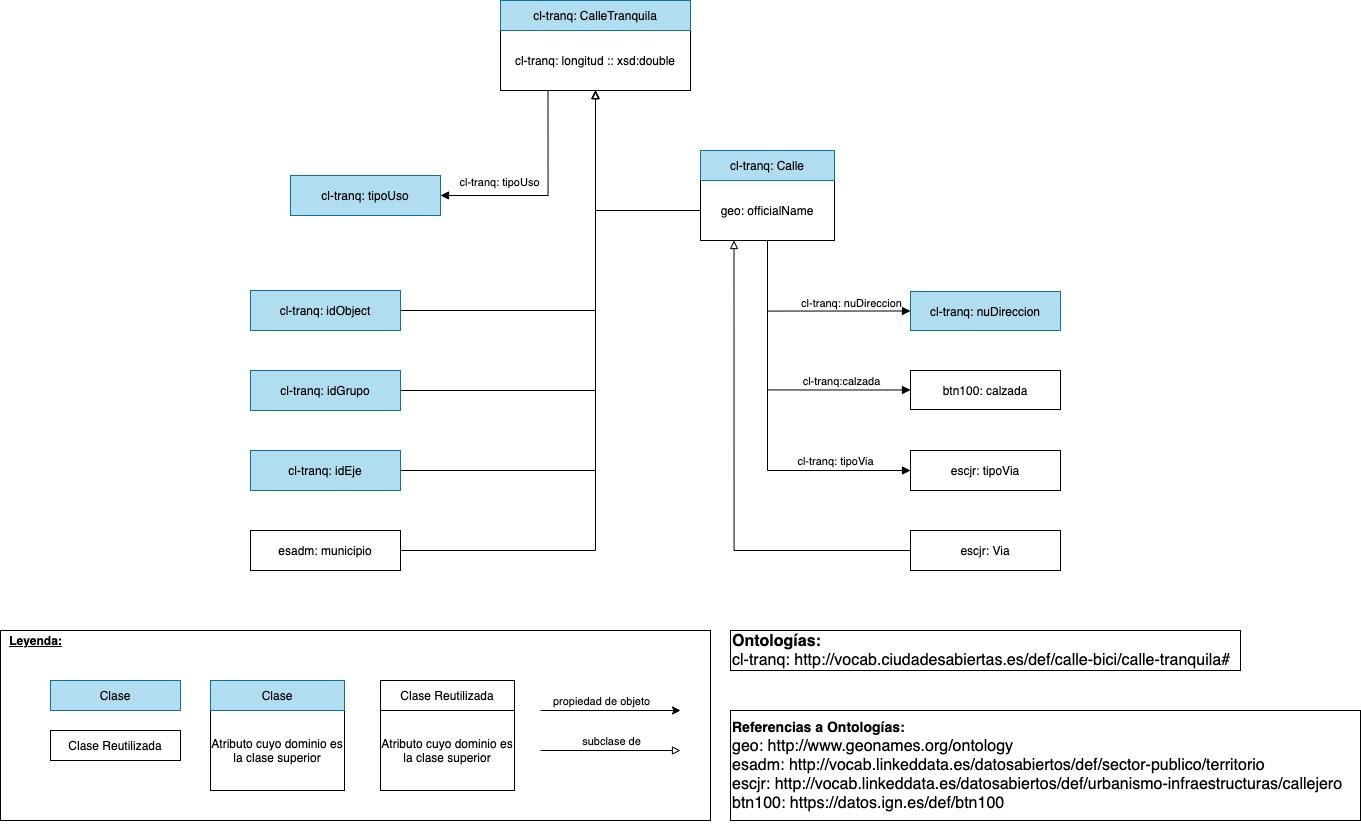
\includegraphics[angle=0, width=0.8\textwidth]{images/diagramaCallesTranqui.png}  
	\caption{Diagrama de Ontología de Calles Tranquilas en Madrid.}
	\label{fig:diagramaOntologCallTranq}
\end{figure}


Para la representación de los datos de calles tranquilas para ciclistas se han definido varias clases y propiedades. Se han tomado como ejemplo el vocabulario definido en ciudades abiertas de Callejero \cite{ciudadesbiertas_callejero} y el definido en datos.ign sobre calzadas \cite{datosIgnCalzada}.
\newline
Se han realizados ciertas modificaciones con respecto al dataset original para que puedan utilizarse sus datos más eficazmente.
Se ha optado por la separación del tipo de via del nombre, conservandola en éste y creando una nueva propiedad que permita saber su clase. Algunos ejemplos serían Calle, Avenida, Plaza...
Se ha añadido el identificador de la via, obtenido a partir del nombre y cruzado con el dataset del callejero de madrid \cite{datosmadrid_callejero}. El identificador permitirá hacer búsquedas mucho más rápidas sobre los datos en caso de querer hacerla filtrando por la calle, que es el caso de la aplicación final que se desea realizar para este proyecto.
En este caso el municipio será siempre madrid, pero en caso de que se quisiera reulizar en otros proyectos a mayor escala sería necesario conocer la zona geográfica donde se encuentra, por tanto también se ha añadido, aunque con el valor fijo de Madrid, que corresponde al código 28079, proporcionado por el Instituto Nacional de Estadistica\cite{datosIgnMunicipios}.

Estas transformaciones se detallarán más adelante en la seccion: Transformaciones en los vocabularios.

Se ha optado por omitir la propiedad ID$\_$TIPO, ya que representa lo mismo que TX$\_$CAPA (el uso que tiene la via) y se ha optado por la segunda por ser representado con texto, más visual y representativo a la hora de su utilización.

El tipo de uso se ha definido en \url{http://vocab.ciudadesabiertas.es/def/calle-bici#tipoUso} debido a que es común para todas las calle-bici (tanto calles tranquilas como ciclocarriles), por lo tanto se ha optado porque los valores sean definidos en una categoria que englobe a las dos.
La dirección se ha definido también en esta categoría común ya que podría ser añadida a ciclocarriles por el ayuntamiento o ser común con otros dataset de una categoría similar( \url{http://vocab.ciudadesabiertas.es/def/calle-bici#nuDireccion} ).

En la siguiente tabla se muestran los Namespaces usados.

\begin{figure}[h]
	\centering
		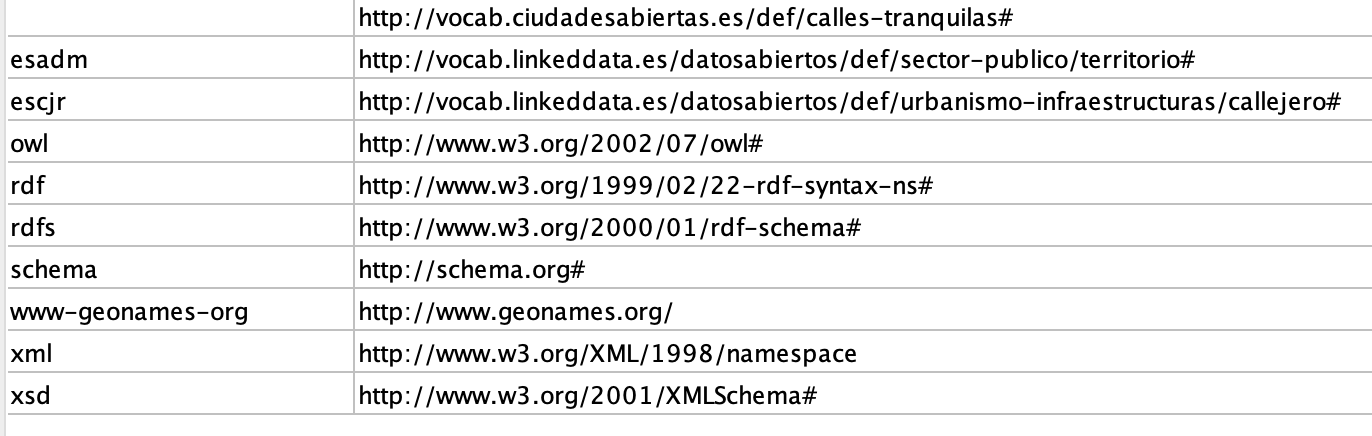
\includegraphics[angle=0, width=0.8\textwidth]{images/tablaIRIsCallesTranquilas.png}  
	\caption{Namespaces usados para Calles Tranquilas}
\end{figure}


Debido a la falta de disponibilidad de una leyenda o información proporcionada por el ayuntameinto de Madrid, para este conjunto de datos no se han podido conocer con exactitud el significado de sus datos. Se ha obtenido de forma aproximada esa información pero podria no ser correcta.


